% (c) 2010 Konstantin Sering <konstantin.sering <aet> gmail.com>
% (cc)-by -- Licenced under Creative Commons Attribution unported
% (http://creativecommons.org/licenses/by/3.0/)
%
\documentclass[xcolor={fixpdftex,hyperref,x11names},10pt,pdftex,hyperref={pdftex}]{beamer}
 
% Pakete
\usepackage[utf8]{inputenc}
\usepackage{lmodern}
\usepackage[T1]{fontenc}
\usepackage[english]{babel}
\usepackage{graphicx}
\usepackage{booktabs}
\usepackage{amssymb}
\usepackage{amsmath}
\usefonttheme[onlymath]{serif}
\usepackage{tikz}
\usetikzlibrary{arrows,shapes}
\usepackage{fancyvrb}
\usepackage{color}
\usepackage{apacite}

%\useoutertheme{tree}
\useinnertheme{circles}
\usecolortheme{orchid}
\usecolortheme{whale}
%\usecolortheme{blue}


% Informationen
\title{Applying IICM to simulated 3D IDM}
\subtitle{ESMP 2013 -- Group 7}
\author{Micha, Michael, Marilisa, Jan, and Tino}
\institute{European Union -- Oulanka Research Station}
\date{23.03.2013}

% Sonstiges
\renewcommand{\emph}[1]{\color{red}#1 \color{black}}


\begin{document}

\maketitle

\begin{frame}
  \frametitle{Outline}
  \tableofcontents
\end{frame}

\begin{frame}
  \frametitle{Todos}
  \begin{itemize}
      \item focus only on SJ3 task
      \item show SJ2 and TOJ in the end (and there only plots)
  \end{itemize}
  \begin{columns}[t]
      \begin{column}{0.5\textwidth}
  \begin{block}{Micha}
      \begin{itemize}
          \item fit data to IICM
          \item slides Motivation + SJ3 task
      \end{itemize}
  \end{block}
  \begin{block}{Marilisa}
      \begin{itemize}
          \item fit data to IICM
          \item slides IICM
      \end{itemize}
  \end{block}
      \end{column}
      \begin{column}{0.5\textwidth}
  \begin{block}{Michael}
      \begin{itemize}
          \item fit data to IICM
          \item slides IDM
      \end{itemize}
  \end{block}
  \begin{block}{Jan}
      \begin{itemize}
          \item Simulate data
      \end{itemize}
  \end{block}
  \begin{block}{Tino}
      \begin{itemize}
          \item Simulate data
      \end{itemize}
  \end{block}
    \end{column}
  \end{columns}
\end{frame}

\section{Motivation}
\label{sec:motivation}

\begin{frame}
  \frametitle{Goal}
  How to combine Ising Decision Model (IDM) and the IICM.

  \begin{itemize}
      \item Insight into the way we did this.
      \item How we approached this?
      \item What resources we had?
      \item What were the steps we take?
  \end{itemize}
\end{frame}

\section{Temporal Judgment Tasks}
\label{sec:tjt}
%\section{Decision Tasks}





\section{Ising Decision Making (IDM)}
\label{sec:idm}





\section{Simulations}
\label{sec:simu}




\section{Integrated Independent Channels Model (IICM)}
\label{sec:iicm}





\section{Fitting the IICM to IDM Data}
\label{sec:fitting}

\subsection{Model Selection}

\begin{frame}
  \frametitle{Model Selection}
  Restricting model parameters in the IICM.

  \begin{itemize}
      \item Parameter..
  \end{itemize}
\end{frame}

\subsection{SJ3 SJ2 TOJ}


%\begin{frame}
%    \frametitle{Three conditions}
%    \begin{columns}
%        \begin{column}{0.6\textwidth}
%    \begin{table}
%        \centering
%        \begin{tabular}{lccc}
%                       & adaptation & ISI    & test \\\hline
%            short prim &  80 ms     & 40 ms  & 0.5 s \\
%            rMAE       &  0.5 s     & 0.25 s & 0.5 s \\
%            long prim  &  0.5 s     & 4 s    & 0.5 s \\\hline
%        \end{tabular}
%        \caption{The different durations for the three experimental
%        conditions in all three experiments.}
%        \label{tab:conditions}
%    \end{table}
%        \end{column}
%        \begin{column}{0.4\textwidth}
%           \includegraphics[width=\textwidth]{./bilder/van_dam_1.pdf}
%        \end{column}
%    \end{columns}
%
%    \begin{block}{Adaptation stimuli}<2->
%        \begin{columns}
%            \hspace{1cm}
%            \begin{column}{.3\textwidth}
%               \includegraphics[width=2cm]{./bilder/adaptation_stim.pdf}
%            \end{column}
%            \begin{column}{.4\textwidth}
%               In all three experiments the adaptation stimuli were
%               white to the right/left moving dots.
%           \end{column}
%        \end{columns}
%    \end{block}
%\end{frame}


\begin{frame}
    \frametitle{Take home message}
  \begin{columns}[t]
      \begin{column}{0.7\textwidth}
        \begin{block}{There is a rMAE, but$\dots$}
            With very short adaptation durations (40 ms to 500 ms) there is
            a motion after effect (rMAE), but it depends on the ISI and the
            test stimulus weather it is a negative or a positive one
            (priming).
        \end{block}

        \vspace{1cm}
        \begin{center}
       \includegraphics[width=2cm]{./bilder/test_stim_ambiguous.png}
       \includegraphics[width=2cm]{./bilder/test_stim_coherence.pdf}
       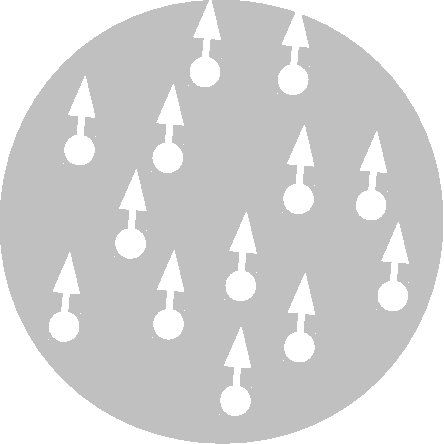
\includegraphics[width=2cm]{./bilder/test_stim_upwards.pdf}
        \end{center}
      \end{column}
      \begin{column}{0.3\textwidth}
        \begin{figure}[h]
          \centering
          \includegraphics[width=\textwidth]{./bilder/waterfall.png}
          \caption{The waterfall illusion is a well known example of the MAE.}
          \label{fig:waterfall}
        \end{figure}
      \end{column}
  \end{columns}
\end{frame}

\begin{frame}{Literatur}
    \nocite{kanai_perceptual_2005}
    \bibliographystyle{apacite}
    \bibliography{talk}
    \normalsize%
\end{frame}

\end{document}

